%% LyX 2.2.2 created this file.  For more info, see http://www.lyx.org/.
%% Do not edit unless you really know what you are doing.
\documentclass[english]{article}
\usepackage[T1]{fontenc}
\usepackage[latin9]{luainputenc}
\usepackage{color}
\usepackage{babel}
\usepackage{float}
\usepackage{graphicx}
\usepackage[unicode=true,pdfusetitle,
 bookmarks=true,bookmarksnumbered=false,bookmarksopen=false,
 breaklinks=false,pdfborder={0 0 0},pdfborderstyle={},backref=false,colorlinks=true]
 {hyperref}

\makeatletter
%%%%%%%%%%%%%%%%%%%%%%%%%%%%%% User specified LaTeX commands.
\usepackage{changepage}
\usepackage{geometry}

\makeatother

\begin{document}
\begin{figure}[t]
\centering{}\includegraphics[scale=0.4]{images/front_page/Logo_polimi_grande}
\end{figure}


\title{{\huge{}Requirements Analysis and Specifications Document}}

\author{\noindent Guido Muscioni (mat. 876151)\\
Marco Orbelli (mat. 876649)\\
Paola Marchesini (mat. 876541)}

\date{\phantom{x}}

\maketitle
\begin{figure}[H]
\begin{centering}
\includegraphics[scale=0.6]{images/Logo}
\par\end{centering}
\caption{New brand logo.}

\end{figure}

\newpage{}

\tableofcontents{}\newpage{}

\section{Introduction}

\section{Architectural design}

\subsection{Overview}

\hfill{}

\,

\paragraph{Logical architecture}

\begin{figure}[H]
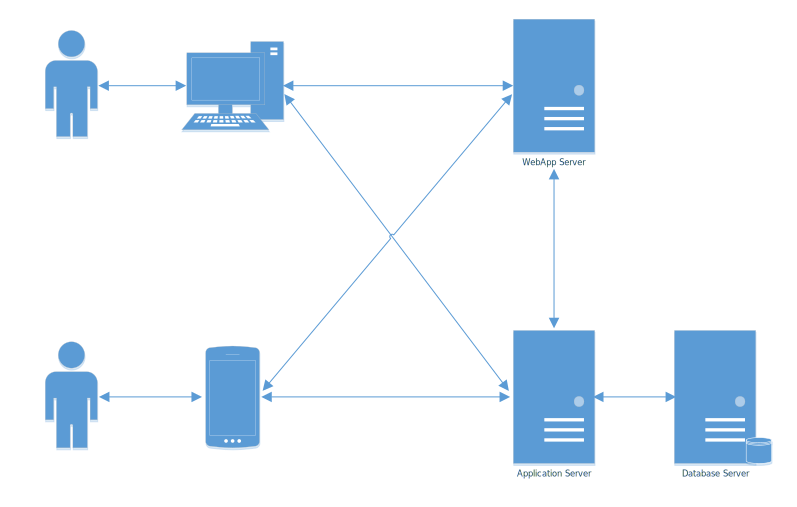
\includegraphics[scale=0.3]{Diagrams/Architecture/Architecture}

\caption{Overview architecture.}

\end{figure}

<TODO: parlare dell'implementazione di un quarto tier adibito alla
business logic. CLOUD?>

The system of PowerEnjoy service is composed by a three layer architecture:
\begin{itemize}
\item Presentation layer: is the tier which allows the general user (employee
and user) of the system to interact with the functionality of PowerEnjoy
service. The users can access to the system with a common web broswer,
or with the mobile application. The web server contains the structure
of the web pages, and it answers to the user's requests, generating
the page with the proper data, received from the application server.
There are two ways of interaction between users and system. The first
one with a modern and up to date web broswer. The second one is represetend
by the mobile application, which is completely derivated from the
website, using Phonegap service to transform it in an executable file
for all the mobile OS nowdays available. Due to that, the website
will be developed following the principles of responsive pages, in
order to reduce the amount of code, and increase the product quality
attributes (as maintainability, performance, portability, etc...).
Furthermore, a responsive design will give to the users of PowerEnjoy
system a service easy to use and always familiar;
\item <TODO: stesso diagramma con DMZ in rosso cos� si capisce meglio>
\item <TODO: server farm con due server per ogni tier tranne il client>
\end{itemize}

\paragraph{Tier architecture}

\begin{figure}
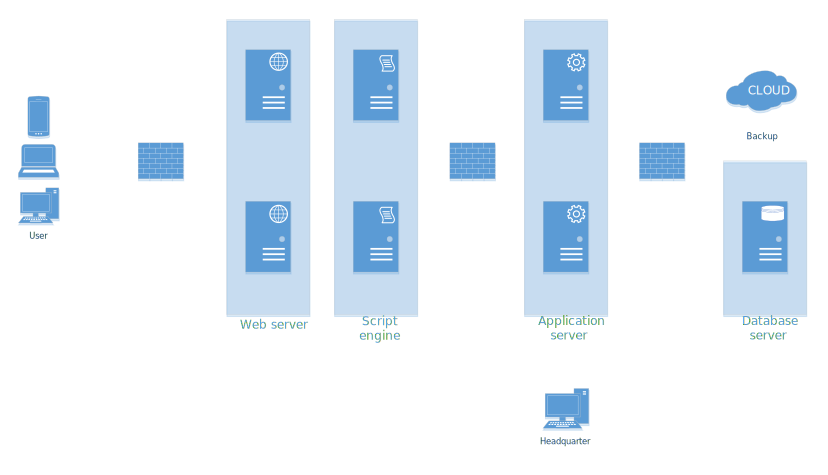
\includegraphics[angle=90,scale=0.5]{Diagrams/Architecture/Architecture_firewall}

\caption{Real architecture of }

\end{figure}

\end{document}
